% Options for packages loaded elsewhere
\PassOptionsToPackage{unicode}{hyperref}
\PassOptionsToPackage{hyphens}{url}
\PassOptionsToPackage{dvipsnames,svgnames*,x11names*}{xcolor}
%
\documentclass[
]{article}
\usepackage{lmodern}
\usepackage{amssymb,amsmath}
\usepackage{ifxetex,ifluatex}
\ifnum 0\ifxetex 1\fi\ifluatex 1\fi=0 % if pdftex
  \usepackage[T1]{fontenc}
  \usepackage[utf8]{inputenc}
  \usepackage{textcomp} % provide euro and other symbols
\else % if luatex or xetex
  \usepackage{unicode-math}
  \defaultfontfeatures{Scale=MatchLowercase}
  \defaultfontfeatures[\rmfamily]{Ligatures=TeX,Scale=1}
\fi
% Use upquote if available, for straight quotes in verbatim environments
\IfFileExists{upquote.sty}{\usepackage{upquote}}{}
\IfFileExists{microtype.sty}{% use microtype if available
  \usepackage[]{microtype}
  \UseMicrotypeSet[protrusion]{basicmath} % disable protrusion for tt fonts
}{}
\makeatletter
\@ifundefined{KOMAClassName}{% if non-KOMA class
  \IfFileExists{parskip.sty}{%
    \usepackage{parskip}
  }{% else
    \setlength{\parindent}{0pt}
    \setlength{\parskip}{6pt plus 2pt minus 1pt}}
}{% if KOMA class
  \KOMAoptions{parskip=half}}
\makeatother
\usepackage{xcolor}
\IfFileExists{xurl.sty}{\usepackage{xurl}}{} % add URL line breaks if available
\IfFileExists{bookmark.sty}{\usepackage{bookmark}}{\usepackage{hyperref}}
\hypersetup{
  colorlinks=true,
  linkcolor=red,
  filecolor=Maroon,
  citecolor=Blue,
  urlcolor=Blue,
  pdfcreator={LaTeX via pandoc}}
\urlstyle{same} % disable monospaced font for URLs
\usepackage[margin=1in]{geometry}
\usepackage{graphicx}
\makeatletter
\def\maxwidth{\ifdim\Gin@nat@width>\linewidth\linewidth\else\Gin@nat@width\fi}
\def\maxheight{\ifdim\Gin@nat@height>\textheight\textheight\else\Gin@nat@height\fi}
\makeatother
% Scale images if necessary, so that they will not overflow the page
% margins by default, and it is still possible to overwrite the defaults
% using explicit options in \includegraphics[width, height, ...]{}
\setkeys{Gin}{width=\maxwidth,height=\maxheight,keepaspectratio}
% Set default figure placement to htbp
\makeatletter
\def\fps@figure{htbp}
\makeatother
\setlength{\emergencystretch}{3em} % prevent overfull lines
\providecommand{\tightlist}{%
  \setlength{\itemsep}{0pt}\setlength{\parskip}{0pt}}
\setcounter{secnumdepth}{-\maxdimen} % remove section numbering
\usepackage{pdfpages}
\usepackage{amsmath}
\usepackage{booktabs}
\usepackage{longtable}
\usepackage{array}
\usepackage{multirow}
\usepackage{wrapfig}
\usepackage{float}
\usepackage{colortbl}
\usepackage{pdflscape}
\usepackage{tabu}
\usepackage{threeparttable}
\usepackage{threeparttablex}
\usepackage[normalem]{ulem}
\usepackage{makecell}
\usepackage{xcolor}
\newlength{\cslhangindent}
\setlength{\cslhangindent}{1.5em}
\newenvironment{cslreferences}%
  {}%
  {\par}

\author{}
\date{\vspace{-2.5em}}

\begin{document}

\pagenumbering{gobble}

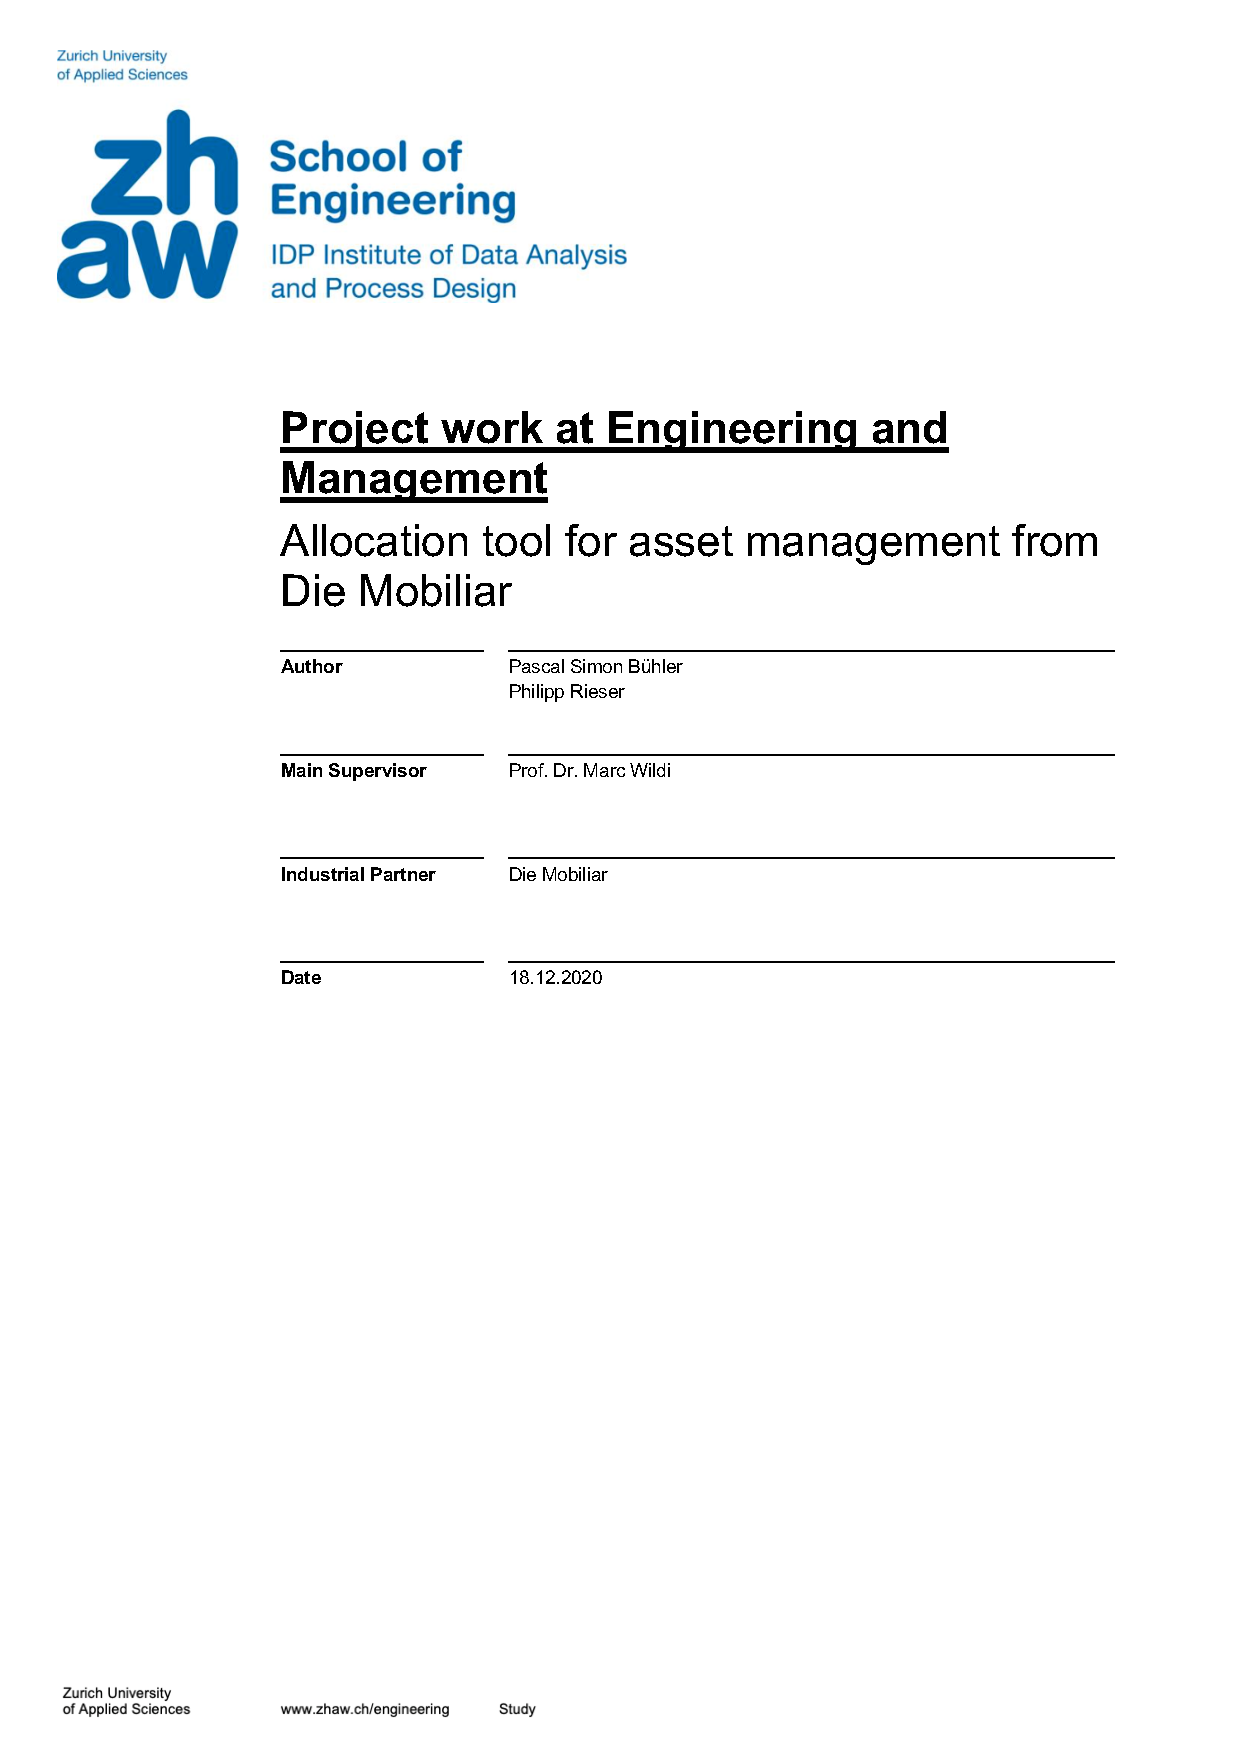
\includepdf{add/titlepage.pdf}

\includepdf{add/declaration.pdf}

\tableofcontents

\newpage

\hypertarget{abstract}{%
\subsection{Abstract}\label{abstract}}

\newpage

\pagenumbering{arabic}

\hypertarget{introduction}{%
\subsection{1. Introduction}\label{introduction}}

The main purpose of trading is buying and selling stocks, bonds, or
other financial instruments with increasing the returns of the
investments in mind while maintaining relatively low risk. With the help
of a trading strategy, an investor can try to improve his performance.
One can simply divide the strategies into passive and active. The
praised and well established passive strategy buy-and-hold takes no
short price movements into account. Positioning and trading based on
these short price movements are considered active trading.

This paper applies time-series analysis to these short price movements
to create active trading strategies. The objective of these developed
strategies is to outperform the buy-and-hold strategy.

\hypertarget{data-analysis}{%
\subsubsection{1.1. Data Analysis}\label{data-analysis}}

The dataset which will be analyzed in this paper contains 4 tradeable
indexes, a visualization of the data is shown below in figure
\ref{fig:chap1.1}.

\begin{figure}

{\centering 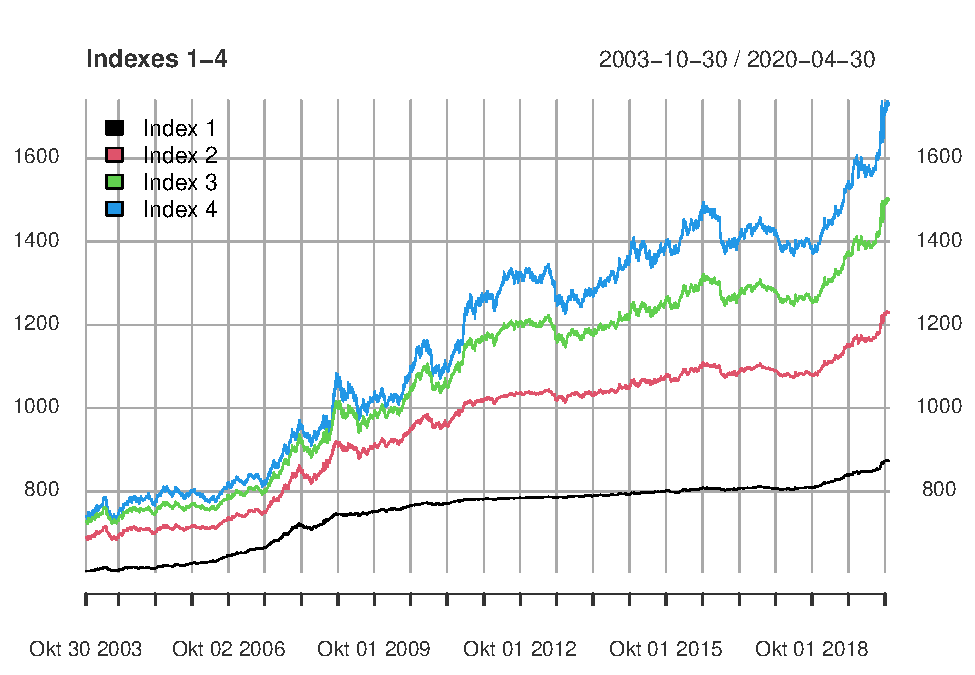
\includegraphics[width=0.7\linewidth]{00_main_files/figure-latex/chap1.1-1} 

}

\caption{Visualization of the 4 indexes}\label{fig:chap1.1}
\end{figure}

Each time-series has 4306 observations and starts from October 2003 to
April 2020. In all indexes is an upward drift observable, during the
time period of the great recession (2008) is a slight bump visible. Also
later in 2013 and 2016 are small break-ins evident. More interesting is
the up and down behavior at the end of the series during the Covid19
pandemic.

\newpage

In addition, to the indexes, the dataset contains 8 different interest
rates of treasury bonds which will be used for further analysis. A few
key-values of the interest rates are shown in the following table
\ref{tab:inttable}.

\begin{table}[!h]

\caption{\label{tab:inttable}Summary of the 8 interest rates.}
\centering
\begin{tabular}[t]{llrrrr}
\toprule
  & Maturity & Mean & Volatility & Min. & Max.\\
\midrule
\cellcolor{gray!6}{Interest 1} & \cellcolor{gray!6}{3M} & \cellcolor{gray!6}{4.09} & \cellcolor{gray!6}{4.95} & \cellcolor{gray!6}{-0.28} & \cellcolor{gray!6}{16.27}\\
Interest 2 & 6M & 4.47 & 5.05 & 0.01 & 16.73\\
\cellcolor{gray!6}{Interest 3} & \cellcolor{gray!6}{1Y} & \cellcolor{gray!6}{4.64} & \cellcolor{gray!6}{4.22} & \cellcolor{gray!6}{0.20} & \cellcolor{gray!6}{10.51}\\
Interest 4 & 2Y & 5.42 & 4.58 & 0.49 & 16.58\\
\cellcolor{gray!6}{Interest 5} & \cellcolor{gray!6}{3Y} & \cellcolor{gray!6}{6.16} & \cellcolor{gray!6}{4.33} & \cellcolor{gray!6}{0.75} & \cellcolor{gray!6}{16.51}\\
\addlinespace
Interest 6 & 5Y & 7.41 & 3.82 & 1.06 & 16.44\\
\cellcolor{gray!6}{Interest 7} & \cellcolor{gray!6}{7Y} & \cellcolor{gray!6}{9.50} & \cellcolor{gray!6}{3.31} & \cellcolor{gray!6}{1.71} & \cellcolor{gray!6}{16.63}\\
Interest 8 & 10Y & 11.61 & 2.93 & 3.13 & 17.47\\
\bottomrule
\end{tabular}
\end{table}

A typical characteristic of interest rates is shown in the given data. A
bond with longer maturities is often associated with higher returns
compared with those with shorter maturities. An investor which invests
in short-term treasury bonds will have his gain earlier but will be
confronted with a lower return.

A more in depth analysis of the given dataset will follow in section
\protect\hyperlink{ts-analysis}{3.1}.

\hypertarget{ojective-of-this-paper}{%
\subsubsection{1.2. Ojective of this
paper}\label{ojective-of-this-paper}}

The objective of this paper is to trade these 4 indexes with an active
trading strategy. The main objective is to outperform the passive
buy-and-hold strategy. Methods such as the Moving-Average-Filter or the
ARMA-GARCH-Model provide signals for either long or short the position
to maximize the return of the investments in these indexes.

The performance of these strategies are build open various different
parameters and conditions. The lengths of the filters applied to a
Moving-Average may result in different solutions. Models could perform
differently for any given length of the in-sample or out-of-sample
scope. The necessity of including a historical crisis in the
starting-sample can decide if a model performs better or worse than
another. The correct validation of model parameters could have a
significant impact on the forecasts.

In addition to all criteria and conditions, the strategies can be
further adjusted by composing different weighted portfolios. Estimated
predicted volatility can be used to modulate the position size to
mitigate the risk.

Challenging will be finding the most optimal model in this wide field of
conditions and parameters. The buy-and-hold strategy will be used as a
benchmark to be compared with the developed active trading strategies.
Computing and comparing the Sharpe ratios of each model can serve as an
indicator to rely on for better or worse models.

\newpage

\hypertarget{theory}{%
\subsection{2. Theory}\label{theory}}

It is assumed that the reader of this paper already has basic knowledge
of the mathematical principles of time series analysis. Therefore, this
section will only briefly describe the mathematical models and
processes.

\hypertarget{time-series}{%
\subsubsection{2.1. Time-Series}\label{time-series}}

Almost anything with a data point to a given timestamp can be named a
time-series. The monthly gross domestic product, the weekly US gasoline
production, or daily stock price movements. In this paper lies the focus
of the analysis of financial time series. Due to trades often only take
place during the week, there are gaps in the time series on the
weekends, an exception would be the trading of cryptocurrencies like
Bitcoin which are also tradeable at the weekends.

A series of data points with more or less equidistant time points \(t\)
with the sample length of \(T\), is called a time-series
\(x_{t}, t=1,...,T\) {[}1{]}. The analysis of a time-series \(x_{t}\)
involves creating a reasonable model that can be utilized to perform
forecast predictions.

\hypertarget{stationarity}{%
\paragraph{2.1.1. Stationarity}\label{stationarity}}

~

In order to fit a suitable model with a given time series \(x_{t}\), the
assumptions of stationarity must be met. In this practical application,
only the following weak-stationarity properties are required.

\begin{equation}
  \label{eq:mean}
  E[x_{t}]=\mu
\end{equation}

\begin{equation}
  \label{eq:var}
  Var(x_{t})=\sigma_{x}^{2}
\end{equation}

\begin{equation}
  \label{eq:cov}
  Cov(x_{t}, x_{t-k})=R(k)
\end{equation}

Many financial time-series are subject to shift, trends or changing
volatility. In figure \ref{fig:chap2.1} are the stock prices of Alphabet
Inc Class A (Google) visualized. This time-series shows a clear upwards
drift and towards the end the volatility increases.

\begin{figure}

{\centering 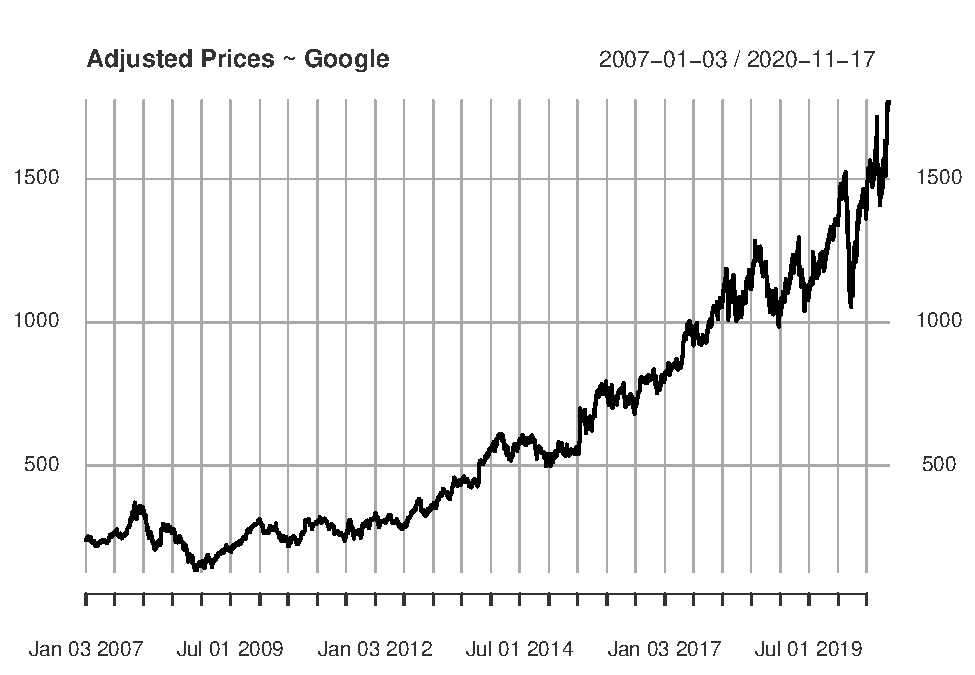
\includegraphics[width=0.7\linewidth]{00_main_files/figure-latex/chap2.1-1} 

}

\caption{Visualization of the adjusted prices of the Alphabet Inc Class A Stock.}\label{fig:chap2.1}
\end{figure}
\newpage

To improve the violated properties the first difference can be applied
and additionally a logarithmic transformation can be performed {[}2{]}.
The log-returns transformation can only performed to strict positive
data.

\[\mathrm{LogReturn} = \mathrm{log}(x_{t})-\mathrm{log}(x_{t-1})\]

The result is the so-called log-returns.

\begin{figure}

{\centering 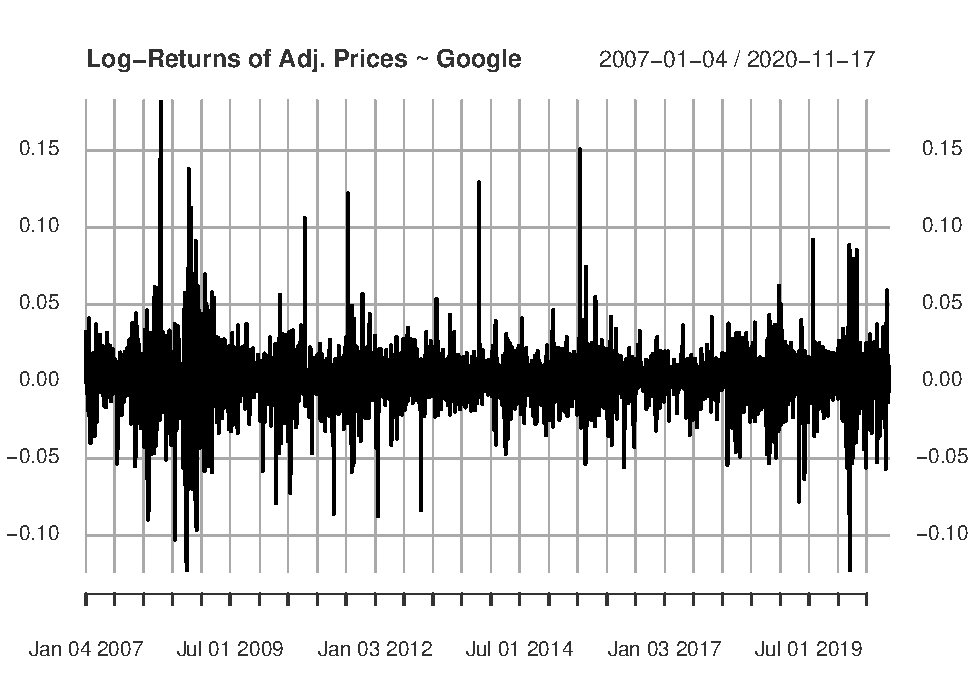
\includegraphics[width=0.7\linewidth]{00_main_files/figure-latex/chap2.2-1} 

}

\caption{Visualization of the Log-Returns}\label{fig:chap2.2}
\end{figure}

Applying the transformation to the data causes the drift to disappear,
but the series still contains stronger and weaker volatile phases. This
effect often occurs in non-stationary financial data and is called
volatility cluster. This special property is used for the modeling of
forecast models, which will be discussed in chapter
\protect\hyperlink{models-section}{2.2}.

In the following examples, we will only work with a section of the time
series, as it often makes no sense to look long into the past. The
further a value lies in the past, the smaller its influence on a future
value will be.

\hypertarget{autocorrelation}{%
\paragraph{2.1.2. Autocorrelation}\label{autocorrelation}}

~

The autocorrelation function (ACF) reveals how the correlation between
any two data points of the time series changes as their separation
changes {[}3{]}. More precisely, acf measures the dependence between
\(x_{t}\) and \(x_{t \pm k}\) at lag \(k\). The partial autocorrelation
(PACF) measures the dependency between \(x_{t}\) and \(x_{t-k}\) at lag
\(k\) {[}1{]}. For stationary time series, ACF can be used to identify
the model order of a MA-process, PACF for AR-processes.

In the following figure \ref{fig:chap2.1.2} are ACF and PACF of the
non-stationary adjusted Google stock visualized. Both graphics show the
typical pattern of a non-stationary time series. The plot above shows
the dependence structure of the time series. This means that it takes a
long time until the series changes. Often a large value is followed by
another large value, which indicates a strong trend. This property of
the series can be seen in figure \ref{fig:chap2.1} as the long upward
drift. The plot below indicates a significant partial autocorrelation at
lag \(k=1\).

In the following section \protect\hyperlink{models-section}{2.2.} the
characteristics of the autocorrelation function can be used for the
verification of ARIMA and ARCH-processes.

\begin{figure}

{\centering 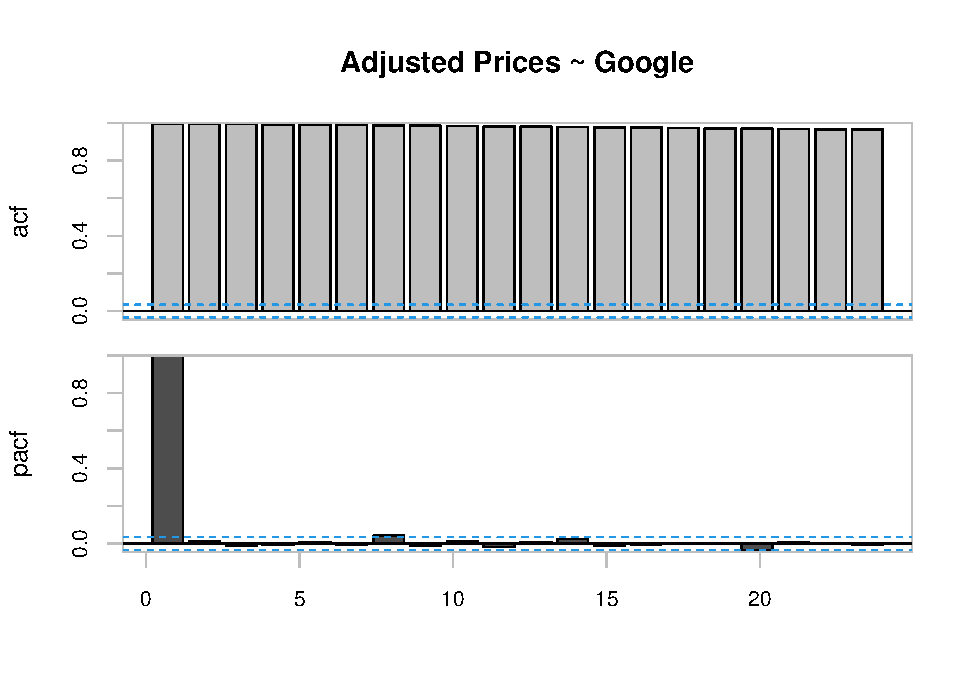
\includegraphics[width=0.7\linewidth]{00_main_files/figure-latex/chap2.1.2-1} 

}

\caption{Acf and Pacf of the Adjusted Prizes of Google.}\label{fig:chap2.1.2}
\end{figure}

\newpage

\hypertarget{models-section}{%
\subsubsection{2.2. Models}\label{models-section}}

The following processes are used to determine certain properties and
characteristics of a time series so that they are transformed into a
model. The goal is to fit the time series as well as possible in order
to create reliable forecasts.

\hypertarget{arima}{%
\paragraph{2.2.1. ARIMA}\label{arima}}

~

An ARIMA(\emph{p},\emph{d},\emph{q}) process is defined as follows.

\begin{equation} \label{eq:arima}
  x_{t}=c+a_{1}x_{t-1}+...+a_{p}x_{t-p}+\epsilon_{t}+b_{1}\epsilon_{t-1}+...+b_{q}\epsilon_{t-q}
\end{equation}

\begin{itemize}
\tightlist
\item
  \(p\) and \(q\) are the AR- and MA-model orders
\item
  \(a\) and \(b\) are the AR- and MA-model parameters
\item
  \(d\) is the differential parameter
\item
  \(\epsilon_t\) is a white noise sequence
\item
  \(x_t\) is the given data \(x_{1},...,x_{T}\)
\end{itemize}

The mean of an ARIMA-process can be computed as:

\[\mu=\frac{c}{1-a_{1}-...-a_{p}}\]

ARIMA processes can be divided into 4 different models. Choosing a model
that best represents the time series is a difficult task. The goal is to
find the best possible model with as few parameters as possible.

The previously introduced ACF and PACF can help to determine the orders
of simple models. Provided that the time series is stationary, the model
orders can be determined directly. For an AR(\emph{p})-process
(ARIMA(\emph{p},\emph{0},\emph{0})), the ACF plot will gradually
decrease and simultaneously the PACF should have a sharp drop after
\emph{p} significant lags. For an MA(\emph{q})-process
(ARIMA(\emph{0},\emph{0}.\emph{q})) the opposite is true, the ACF should
show a sharp drop after a certain \emph{q} number of lags while PACF
should show a gradual decreasing trend. If both ACF and PACF show a
gradual decreasing pattern, then the
ARIMA(\emph{p},\emph{0},\emph{q})-process should be considered for
modeling {[}4{]}. If the time series is not stationary, differentiation
can be considered (ARIMA(\emph{p},\emph{d},\emph{q})).

\newpage

The application of an analysis method to Google prices finds an
ARIMA(\emph{1},\emph{1},\emph{0}) as the optimal model. This makes sense
if you look back at figure \ref{fig:chap2.1.2}. Long dependency
structures in the ACF plot indicating an AR(\emph{p}) process and at the
same time after lag=\(1\)=\emph{p} the PACF has a strong drop. The
differential operator \emph{d}=\(1\) transforms the non-stationary
series into a stationary one.

To convince yourself of the quality of the model, you can use the
Ljung-Box statistics shown in figure \ref{fig:chap2.2.1_1}. For the lags
where the p-values are above the 5\% line, the forecasts are reliable.
Here the values from the 6 lag are below the significant line, but since
one only wants to make short-term forecasts (for example 1 day into the
future), the lag is sufficient up to 5. If you want to forecast further
than 5 days into the future, you might have to adjust the ARIMA model.

\begin{figure}

{\centering 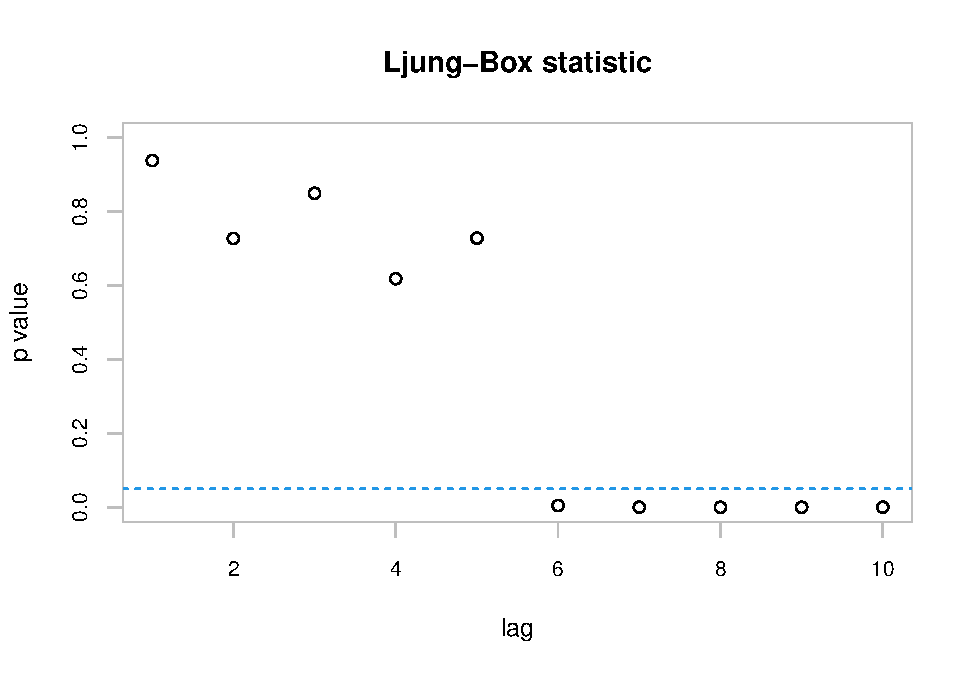
\includegraphics[width=0.7\linewidth]{00_main_files/figure-latex/chap2.2.1_1-1} 

}

\caption{Ljung-Box statistic of Google log returns.}\label{fig:chap2.2.1_1}
\end{figure}

In figure \ref{fig:chap2.2.1_2} you can see the prediction of the model.
The whole representation is shifted by one day so that one can compare
the model with a true value. The \textcolor{green}{green dot} is the
actual value of the time series. The \textcolor{red}{red dots} indicate
the upper and lower 95\% interval limits respectively. These indicate
that a future value will be within this band. The
\textcolor{blue}{blue dot} is the point forecast predicted by the model.

\newpage

\begin{figure}

{\centering 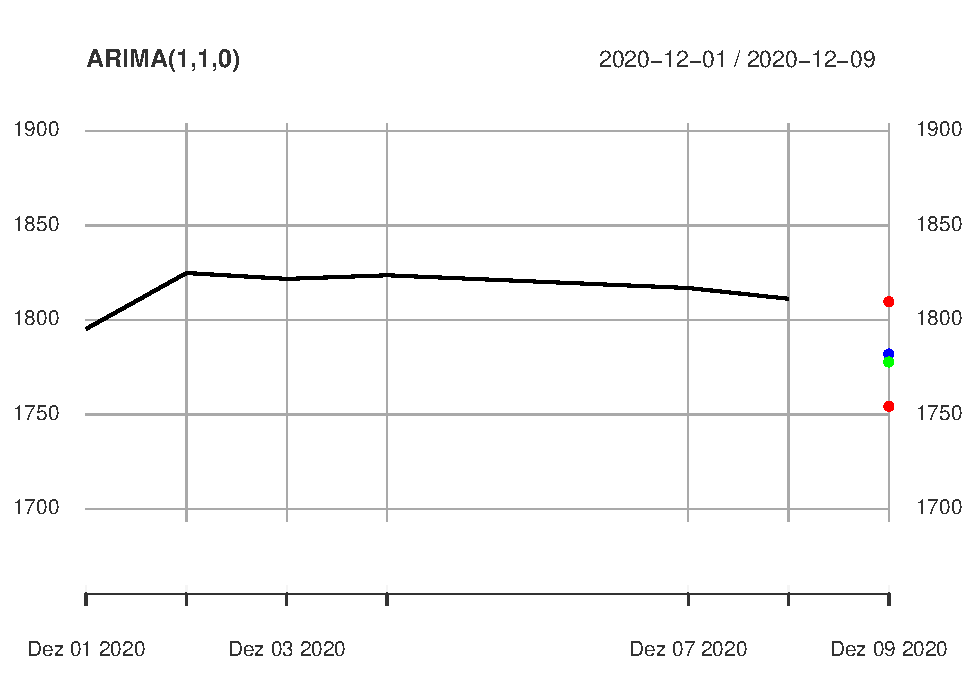
\includegraphics[width=0.7\linewidth]{00_main_files/figure-latex/chap2.2.1_2-1} 

}

\caption{ARIMA-Forecast.}\label{fig:chap2.2.1_2}
\end{figure}

\hypertarget{garch-section}{%
\paragraph{2.2.2. GARCH}\label{garch-section}}

~

The volatility clustering mentioned in section
\protect\hyperlink{stationarity}{2.1.1} can be handled with an
generalized auto-regressive conditional heteroscedastic process.

\begin{align} \label{eq:garch}
  \epsilon_{t} &= \mathrm{log}(x_{t})-\mathrm{log}(x_{t-1}) \nonumber \\
  \epsilon_{t} &= \sigma_{t}u_{t} \\
  \sigma_{t}^{2} &=c \sigma^{2}+\sum_{j=1}^{n}\alpha_{j}\sigma_{t-j}^{2}+\sum_{k=1}^{m}\beta_{k}\epsilon_{t-k}^{2} \nonumber
\end{align}

with

\begin{itemize}
\tightlist
\item
  \(x_{t}\) is the original data (often non-stationary)
\item
  \(\epsilon_{t}\) is the stationary log-return
\item
  \(u_{t}\) is independent and identically distributed (iid) and a
  standardized random variable
\item
  \(\sigma^{2}\) is the unconditional variance of the process
  \(\epsilon_{t}\).
\item
  \(\sigma_{t}^{2}\) is the conditional variance of the process
  \(\epsilon_{t}\).
\end{itemize}

With a GARCH(\emph{n},\emph{m})-process it is possible to model the
volaclusters of a time series. The GARCH(\emph{1},\emph{1}) model has
become widely used in financial time series modeling and is implemented
in most statistics and econometric software packages. Those models are
favored over other stochastic volatility models by many economists due
to their relatively simple implementation {[}5{]}.

\newpage

For an optimal model some conditions must be fulfilled. Suppose you want
to model the Google time series with a GARCH(\emph{1},\emph{1}).

In table \ref{tab:coeftable} the estimated coefficients of the process
can be seen. The p-values are all lower than 0.05 and thus indicate that
they are essential for the model. (Note: \(\omega=c\sigma^{2}\))

\begin{table}

\caption{\label{tab:coeftable}Coefficients GARCH(1,1).}
\centering
\begin{tabular}[t]{lrrr}
\toprule
  & Estimate & Std. Error & p-Value\\
\midrule
$\omega$ & 1.091662e-05 & 1.847832e-06 & 3.467047e-09\\
$\alpha_{1}$ & 7.379179e-02 & 1.081489e-02 & 8.905765e-12\\
$\beta_{1}$ & 8.948648e-01 & 1.380342e-02 & 0.000000e+00\\
\bottomrule
\end{tabular}
\end{table}

The following parameter restrictions are also examined:

\begin{equation} \label{eq:para_restriction}
  c+\sum_{j=1}^{n}\alpha_{j}+\sum_{k=1}^{m}\beta_{k}=1
\end{equation}

with

\[c>0, \alpha_{k}\geq0, j=1,...,n, \beta_{k}\geq0, 1,...,m \]

To satisfy formula \ref{eq:para_restriction}, \(c\) needs to be
determined from \(\omega\). First calculate the unconditional variance.

\[\sigma^{2} = \frac{\omega}{1-\alpha_{1}-\beta_{1}}\]

Calculate \(c\) with:

\[c=\frac{\omega}{\sigma^{2}}\]

and then check for the restriction in \ref{eq:para_restriction}.

For the coefficients of GARCH(\emph{1},\emph{1}) the restrictions are
fulfilled. You can see that \(c = 1-\alpha_{1}-\beta_{1}\). So this
restriction can be determined easily with:

\begin{equation} \label{eq:para_moments_easy}
  \sum_{j=1}^{n}\alpha_{j}+\sum_{k=1}^{m}\beta_{k} < 1
\end{equation}

If the parameter restrictions are not fulfilled, complications may
arise, the forecast of the conditional variance \(\hat{\sigma}^{2}_{t}\)
may diverge to the unconditional variance \(\sigma^{2}\) of the process.

\newpage

Furthermore, the Ljung-Box statistics are important for the standardized
residuals. Looking back at formula \ref{eq:garch} standardized residuals
\(u_{t}\) are proportional to the conditional volatilities
\(\sigma_{t}\), which should lead to the log returns \(\epsilon_{t}\).
The conditional volatilities map the volacluster in the time series. To
achieve the best possible model, one does not want to find these
volacluster effects in the standardized residuals, but only in the
conditional volatilities. The Ljung-Box statistics check this property.
In figure \ref{fig:chap2.2.2} Ljung-Box statistics of the
\(\hat{u}_{t}\) and the \(\hat{u}^{2}_{t}\) are shown.

\begin{figure}

{\centering 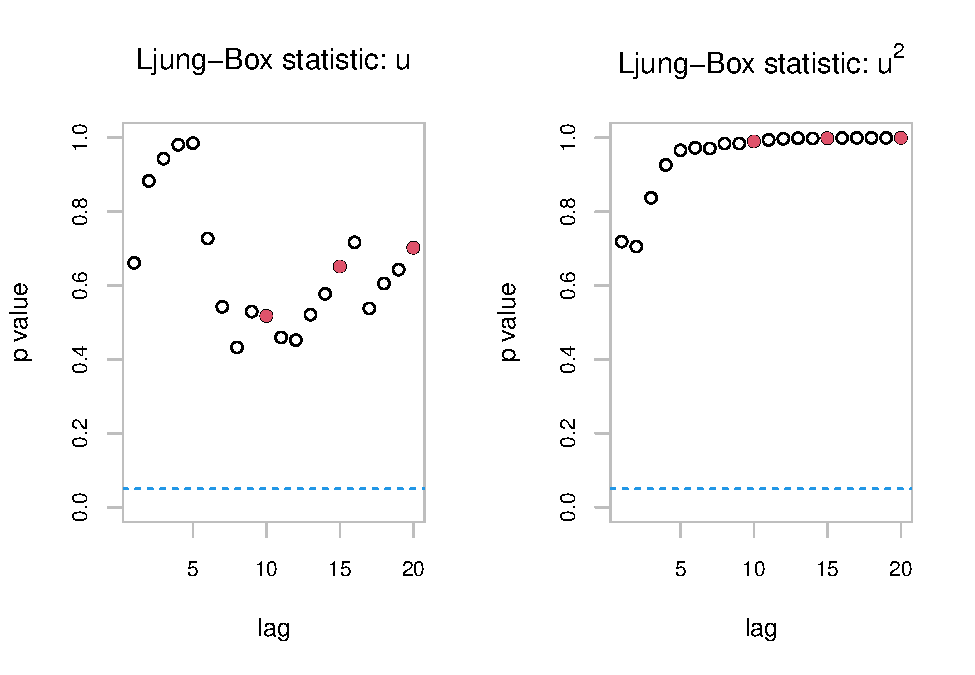
\includegraphics[width=0.7\linewidth]{00_main_files/figure-latex/chap2.2.2-1} 

}

\caption{Ljung-Box statistic of the standardized residuals.}\label{fig:chap2.2.2}
\end{figure}

The plot shows reliable statistics for forecasts from the
Google-GARCH(\emph{1},\emph{1}) model. For all lags up to 20, the
p-values are above the 5\% line and thus hypothesis tests are discarded.
However, if for a given lag=k the p-values would fall below the 5\%
line, then forecasts would only be reliable up to a forecast horizon k.

If one wants to improve the the standardized residuals \(\hat{u}_{t}\)
(if autocorrelations exists in the \(\hat{u}_{t}\)), an ARMA part would
have to be added to the existing model (see
\protect\hyperlink{arma-garch-section}{2.2.3}). This can again be
optimized with different model orders. If you want to improve the
squared standardized residuals \(\hat{u}^{2}_{t}\) (if volaclustering
exists within the \(\hat{u}^{2}_{t}\)), then you should modify the GARCH
model order.

Now an optimal model has been found and a forecast can be made. Since a
GARCH(\emph{n},\emph{m}) process is white noise sequence the expected
value \(E[\epsilon_{T+h} | \epsilon_{T},...,\epsilon_{1}]=\mu=0\) can be
assumed (if the mean value in the fit object was also estimated and is
significant, then the expected value is the estimated \(\mu\)).

Calculating the forecast variance is a recursive process. With
increasing model order the calculation becomes more and more difficult.
For this work the rather simple calculation for a
GARCH(\emph{1},\emph{1}) model is sufficient. One receives:

\[\hat{\sigma}_{T+h}^{2}=\omega+(\alpha_{1}+\beta_{1})^{2}\hat{\sigma}_{T+h-1}^{2}\]

If the parameter restriction from formula \ref{eq:para_moments_easy} is
true, the forecast variance converges with the increasing forecast
horizon to the unconditional variance of the process.

\[\hat{\sigma}_{T+h}^{2}=\frac{\omega}{1-\alpha_{1}-\beta_{1}}=\sigma^{2}\]

\newpage

The 95\% forecast interval is calculated as follows:

\[E[\epsilon_{T+h} | \epsilon_{T},...,\epsilon_{1}]\pm 1.96\sqrt{\hat{\sigma}_{T+h}^{2}}\]

Figure \ref{fig:chap2.2.3} shows the GARCH(\emph{1},\emph{1}) forecast
for 20 days. The blue line represents the expected value of the time
series. Reds are the two 95\%-interval limits and green shows the actual
values of the series.

\begin{figure}

{\centering 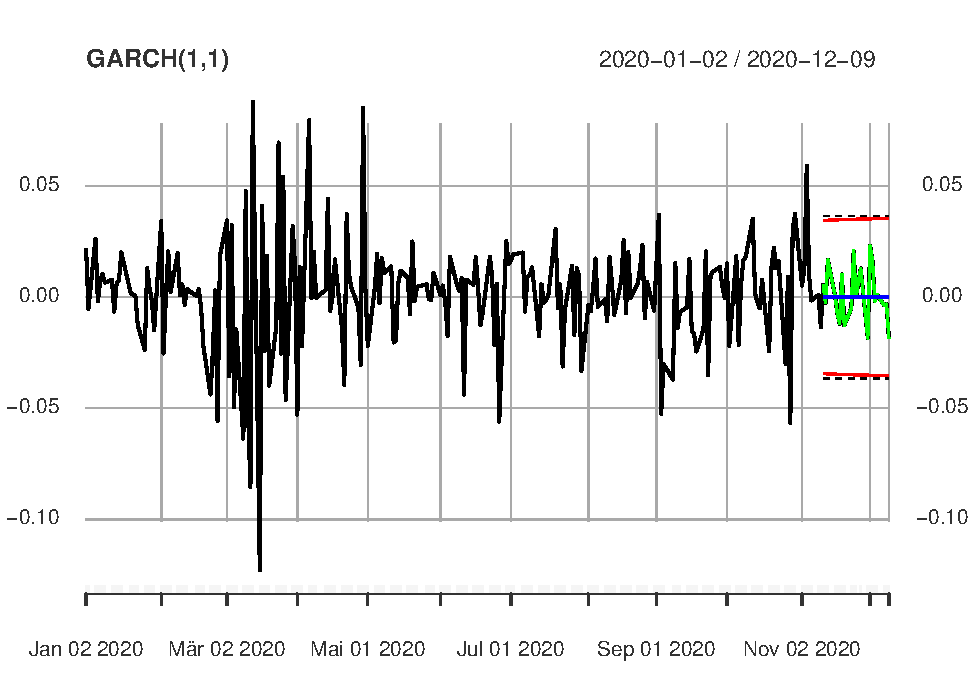
\includegraphics[width=0.7\linewidth]{00_main_files/figure-latex/chap2.2.3-1} 

}

\caption{GARCH-Forecast.}\label{fig:chap2.2.3}
\end{figure}

You can see how the red lines are approaching the black dotted lines
(\(0 \pm 1.96*\sqrt{\sigma^{2}}\)) as the forecast horizon increases.
This means that the forecast variance converges to the unconditional
variance and thus there is another proof for the satisfaction of the
parameter restrictions.

\hypertarget{arma-garch-section}{%
\paragraph{2.2.3. ARMA-GARCH}\label{arma-garch-section}}

~

If you want to adopt a GARCH model and you discover non-vanishing
autocorrelations in the standardized residuals \(\hat{u}_{t}\), the
model can be extended with an ARMA part to counteract the
autocorrelations.

\begin{eqnarray}
y_{t}&=&\mu + a_{1}y_{t-1}+...+a_{p}y_{t-p}+\epsilon_{t}+b_{1}\epsilon_{t-1}+...+b_{q}\epsilon_{t-q} \label{eq:arma-garch1} \\
\epsilon_{t}&=&\sigma_{t}u_{t} \nonumber \\
\sigma_{t}^{2}&=&c\sigma^{2}+\sum_{j=1}^{n}\alpha_{j}\sigma_{t-j}^{2}+\sum_{k=1}^{m}\beta_{k}\epsilon_{t-k}^{2} \label{eq:arma-garch2}
\end{eqnarray}

This model contains now 4 different model orders:
\emph{p},\emph{q},\emph{n} and \emph{m}. Experience shows that for
financial time series, a model order of \emph{n}=\emph{m}=\(1\) and
\emph{p},\emph{q}\(\leq 1\) is often sufficient to fit the data to an
ARMA-GARCH model.

The equation \ref{eq:arma-garch1} is called the \emph{mean-equation} and
describes the conditional mean of the process, which is used to obtain
optimal point forecast. The equation \ref{eq:arma-garch2} defines the
variance of the process and is called \emph{variance-equation}, which is
used for the forecast error variance {[}6{]}.

\newpage

\hypertarget{m-garch}{%
\paragraph{2.2.4. M-GARCH}\label{m-garch}}

~

The last model that is considered as a forecast model in this thesis is
the so-called MGARCH model. Highly volatile phases indicate downturns.
Market participants tend to oversell during these downturns. Overselling
leads to inflated volumes and this in turn leads to inflated
volatilities. This model can be helpful since it emphasizes recession
and crisis dynamics.

\begin{align} \label{eq:mgarch}
  r_{t} &= \mathrm{log}(x_{t})-\mathrm{log}(x_{t-1}) \nonumber \\
  r_{t} &= \mu+e\sigma_{t}+\epsilon_{t} \\
  \epsilon_{t} &= \sigma_{t}u_{t} \nonumber
\end{align}

where

\begin{itemize}
\tightlist
\item
  \(x_{t}\) is the original data (typically non-stationary)
\item
  \(r_{t}\) are the log-returns (stationary)
\item
  \(\mu\) is the long-term drift
\item
  \(\epsilon_{t}\) is a volacluster process (GARCH)
\item
  \(e\) is a constant (a parameter to be estimated), \(e>0\) implies a
  larger expected return. \(e<0\) would imply a smaller expected return.
  If \(e=0\) then the MGARCH-effect vanishes {[}7{]}.
\end{itemize}

For this model, the in-sample conditional standard deviations
(volatilities) from any GARCH process are determined and the
out-of-sample conditional standard deviation for obtaining forecasts of
the future returns is then calculated by regression.

\[\hat{r}_{t+1}=\hat{\mu}+\hat{e}\hat{\sigma}_{t+1}\]

\newpage

\hypertarget{moving-average-filters}{%
\subsubsection{2.3. Moving Average
Filters}\label{moving-average-filters}}

Moving average filters are basically used to identify trends and smooth
out price fluctuations. As a commonly used tool, moving average filters
are very simple in their usage, historical data from a timeframe L gets
summarized and divided by the length of the filter (L). Depending on the
length of the filter, the application to the timeseries the MA gets
shifted, longer filters have a higher shift then shorter ones we
visualize this behavior in \ref{fig:chap2.3.3}. Many different
indicators are built upon the Moving Average principle, mostly they are
used in combinations of different lengths to create signals. In the
following section, we introduce some of the most popular indicators
based on the MA principle.

The actual challenge in using Moving average filters, is to figure out
which length of the filter brings the most useful information.

\hypertarget{equally-weighted-moving-average-or-sma}{%
\paragraph{2.3.1. Equally-weighted Moving Average or
SMA}\label{equally-weighted-moving-average-or-sma}}

~

SMA stands for Simple Moving Average, depending on the length of the
filter(L), L observations since the last noted observation will be
considered. The observations are getting summarized and divided by the
filterlength L. As stated in the name, all past observations are
weighted equally. For every timestep, a new observation is considered
and the last one eliminated {[}8{]}. SMA's are very easily customized by
changeing the length of the filter.

EqMA

\begin{equation}
  \label{eq:eqma}
  y_{t}=\frac{1}{L}\sum_{k=0}^{L-1}x_{t-k}
\end{equation}

\begin{itemize}
\tightlist
\item
  \({L}\) = filterlength
\item
  \({x}\) = original series price e.g.
\end{itemize}

\hypertarget{momentum}{%
\subparagraph{2.3.1.1 Momentum}\label{momentum}}

Momentum is an indicator wether a market is bullish or bearish, it
measures the ``speed'' of the trend direction in the market. for a
timespan \(k\) the last price \(p_k\), \(k\) timesteps ago is subtracted
from the last price. This is equivalent to applying and EqMA on the
returns of a series.

Momentum

\begin{equation}
  \label{eq:momentum}
  y_{t}=p_t - p_{t-K}
\end{equation}

\begin{itemize}
\tightlist
\item
  \({p_t}\) = prices of the series
\item
  \({K}\) = Lag
\end{itemize}

\newpage

\hypertarget{exponentially-weighted-moving-average}{%
\paragraph{2.3.2. Exponentially-weighted Moving
Average}\label{exponentially-weighted-moving-average}}

~

Since not all observations are having the same influence on the future
value, we can apply a weight to past observations. One method will be
exponentially weighted Moving average. So we chose an optimal parameter
to give past observations weights decreasing by \(\alpha^{k}\). In
comparison to the SMA \protect\hyperlink{SMA}{2.3.1.} {[}9{]} ,a EMA
from the same length L, reacts faster than to price changes.

A skillful trader chooses an optimal \(\alpha\) to increase the
performance of the measurement. Weights could also be given individually
by adding a weight vector to the filter.

EMA

\begin{equation}
  \label{eq:ema}
  y_{t}=\frac{1}{\sum_{k=0}^{m}\alpha^{k}}\sum_{k=0}^{m}\alpha^{k}x_{t-k}
\end{equation}

\begin{itemize}
\tightlist
\item
  \({m}\) = filterlength
\item
  \({\alpha}\) = Parameter to weigh the observations
\end{itemize}

~

\hypertarget{moving-average-crossings}{%
\paragraph{2.3.3. Moving Average
Crossings}\label{moving-average-crossings}}

~

Moving average crossings are basically just different MA's with
different lengths applied to a time-series. The points the filters then
cross, will be used as a trading signal to go long, short or hold. The
``death'' and ``golden'' cross are very popular trading patterns
{[}9{]}. If a shorter MA crosses the longer MA from above, its called a
``golden cross'' it is an indicator that the price will rise in the
future and can be used to created the buy signal. In contrast stands the
``death cross'' vise versa, a shorter MA (popular L = 50) crosses a
longer MA(popular L = 200) from below, signalizing that further losses
are in store.

Moving Average Crossing

\begin{equation}
  \label{eq:mac}
  y_{t}=\frac{1}{L_1}\sum_{k=0}^{L_1-1}x_{t-k} - \frac{1}{L_2}\sum_{k=0}^{L_2-1}x_{t-k}
\end{equation}

\begin{itemize}
\tightlist
\item
  \({L_1}\) = filterlength 1
\item
  \({L_2}\) = filterlength 2
\item
  \({0 < \alpha < 1}\) = Parameter to weigh the observations
\end{itemize}

\newpage

An example of MA average crossings with 2 SMAs of different length is
visualized in figure \ref{fig:chap2.3.3}. The prices are in
\textcolor{green}{green} while the \textcolor{blue}{blue line}
represents an \textcolor{blue}{50} day SMA an the
\textcolor{red}{red line} a \textcolor{red}{250 (1 year)} SMA. The
crossing points of those two SMAs could now be used as trading signals.
In this example these crossings wouldn't perform very well, therefore as
mentioned earlier, finding the right length of the filter depends on
each timeseries, their behavior and the preferences of the trader.

~

\begin{figure}

{\centering 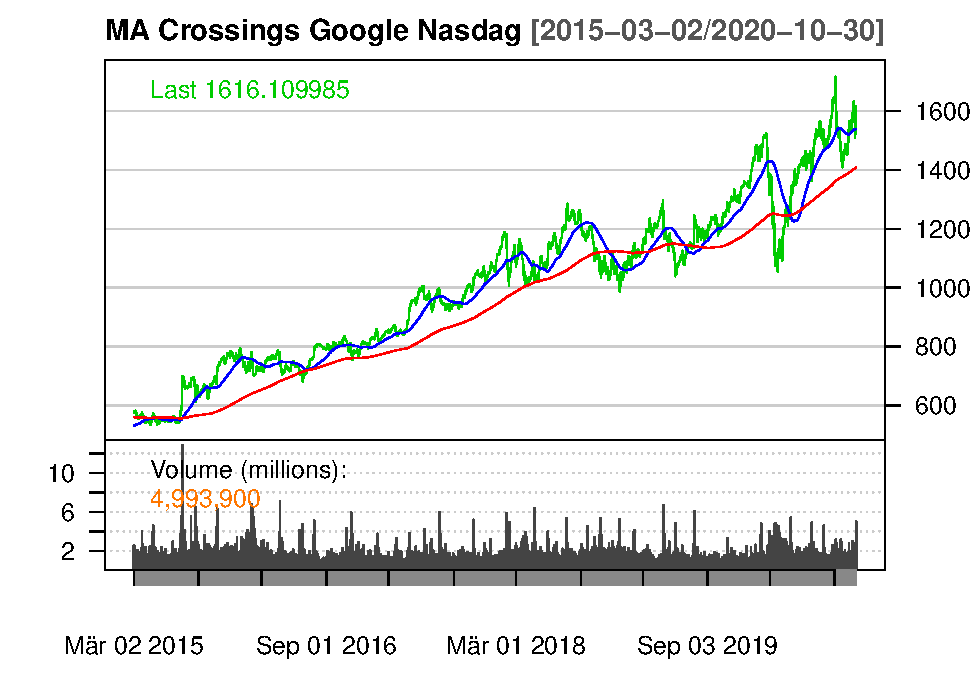
\includegraphics[width=0.7\linewidth]{00_main_files/figure-latex/chap2.3.3-1} 

}

\caption{Moving Average Crossing}\label{fig:chap2.3.3}
\end{figure}

\newpage

\hypertarget{relative-strength-index}{%
\subsubsection{2.4. Relative Strength
Index}\label{relative-strength-index}}

~

The Relative strength index is a tool to measure momentum, the value
indicates if positions are overvalued or undervalued. the scale goes
from 0 to 100. {[}10{]}.

\begin{equation}
  \label{eq:mac1}
  U_{t}=\begin{cases}1, \textnormal{if }    x_t \ge x_{t-1}\\0, \textnormal{otherwise} \end{cases}
  D_{t}=\begin{cases}1, \textnormal{if }  x_t < x_{t-1}\\0, \textnormal{otherwise} \end{cases}
\end{equation}

\begin{itemize}
\tightlist
\item
  \({X_t}\) =Original timeseries
\end{itemize}

We then apply SMA or EMA of length N to \(U_t\) and \(U_t\) which
converts them in \(up_t(N)\) and \(down_t(N)\) The RSI is now computet
by: \begin{equation}
  \label{eq:mac2}
 RSI_t(N)=100\frac{up_t(N)}{up_t(N)+down_t(N)}
\end{equation}

The original developer J. Welles Wilder Jr.~proposed a length of N =14
in its work from 1978 {[}11{]}. Traditional tradings signals based on
the RSI are the upper 70 or lower 30 limit to buy or sell. Usually when
the RSI is going over 70 it suppose that the asset is overvalued and in
contrast when its under 30 then its undervalued.

~

\begin{figure}

{\centering 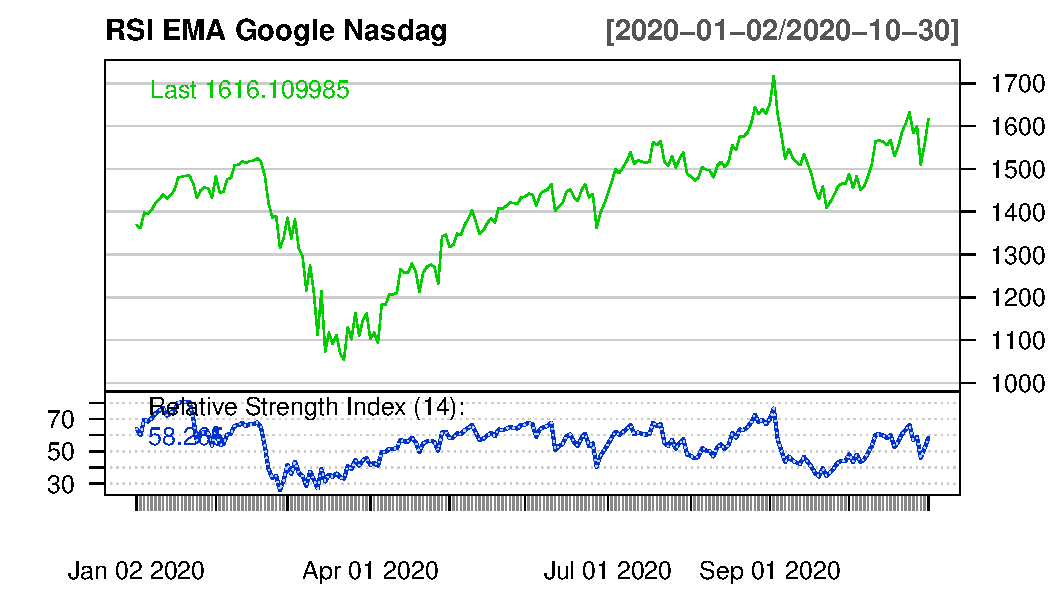
\includegraphics[width=0.7\linewidth]{00_main_files/figure-latex/chap2.4 -1} 

}

\caption{RSI}\label{fig:chap2.4 }
\end{figure}
\newpage

\hypertarget{moving-average-convergence-divergence}{%
\subsubsection{2.5. Moving Average Convergence
Divergence}\label{moving-average-convergence-divergence}}

~ The MACD is also a commonly used filter. The basic principle is to
Subtract a longer EMA with length \(L\) as in section
\protect\hyperlink{EMA}{2.3.3} from a shorter EMA from length \(S\) then
smooth the result with another EMA with length \(R\). As a result with
can use the crossing of the 2 generated curves for trading. As an
alternative we could use SMA's instead of EMA's

\begin{equation}
  \label{eq:MACD}
  \mathrm macd_t =\frac{1}{\sum_{k=0}^{t-1}\alpha^{k}} \sum_{k=0}^{t-1}\alpha^{k}x-{t-k}-\frac{1}{\sum_{k=0}^{t-1}\beta^{k}}\sum_{k=0}^{t-1}\beta^{k}x-{t-k}
\end{equation}

\begin{equation}
  \label{eq:signal MACD}
\mathrm  MACD signal_t=   \frac{1}{\sum_{k=0}^{t-1}\gamma^{k}}\sum_{k=0}^{t-1}\gamma^{k}x-{t-k}
\end{equation}

\begin{itemize}
\tightlist
\item
  \(x_t\) = prices or log prices
\item
  \(S\) = length of the \(short_1\) EMA usually 12
\item
  \(L\) = length of the \(long_1\) EMA usually 26
\item
  \(R\) = length of the ``double smoothing ema'' usually 9
\item
  \(\alpha\) = \(1-\frac{1}{S}\), \(\beta\) = \(1-\frac{1}{L}\),
  \(\gamma\) = \(1-\frac{1}{R}\)
\end{itemize}

\(_1\) short and long in the meaning s\textless l, not buy sell

~

\begin{figure}

{\centering 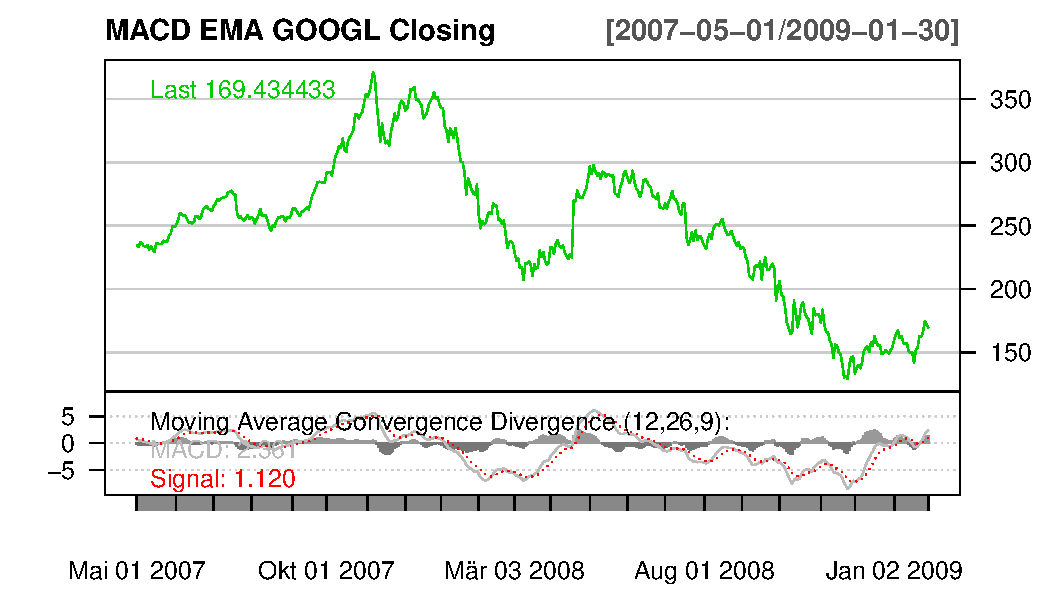
\includegraphics[width=0.7\linewidth]{00_main_files/figure-latex/chap2.5-1} 

}

\caption{MACD}\label{fig:chap2.5}
\end{figure}
\newpage

\hypertarget{bollinger-bands}{%
\subsubsection{2.6. Bollinger bands}\label{bollinger-bands}}

~ Bollinger bands are a analysis tool founded by John Bollinger. It
contains a moving average and an upper and lower band . The bands are
defined by adding a constant \({K}\) times a standard deviation
\({\sigma_t}\) to the \emph{Moving Average} for the upper , and
subtracting it for the lower band.

\begin{equation}
  \label{eq:lower and upper bollingerbands}
  \mathrm{U_t}=MA_{t}+K\sigma, L_{t}=MA_{t}-K\sigma
\end{equation}

the variance from bollingers theory is calculated by:

\begin{equation}
  \label{eq:variance bollingerbands}
  \mathrm{\sigma_{t}^2}=\frac{1}{N}\sum_{k=0}^{N-1}(x_{t-k} -MA_t)^2
\end{equation}

The calculated \({\sigma_t}\) could be problematic because its derived
from the original series and increases with the level, its non
stationary. Therefore an other method to calculate the standard
deviation could be used. As done in section
\protect\hyperlink{garch-section}{2.2.2.} \(\sigma_t\) could be provided
by a GARCH, which would handle the increasing volatility.

\begin{itemize}
\tightlist
\item
  \({N}\) = usually the filterlength and the length considered for
  \({\sigma}\) are the same
\item
  \({K}\) = Constant usually equals 2
\item
  \(\sigma_p\) = standard deviation of the series
\item
  \({U_t}\) = upper band
\item
  \({L_t}\) = lower band
\end{itemize}

~

\begin{figure}

{\centering 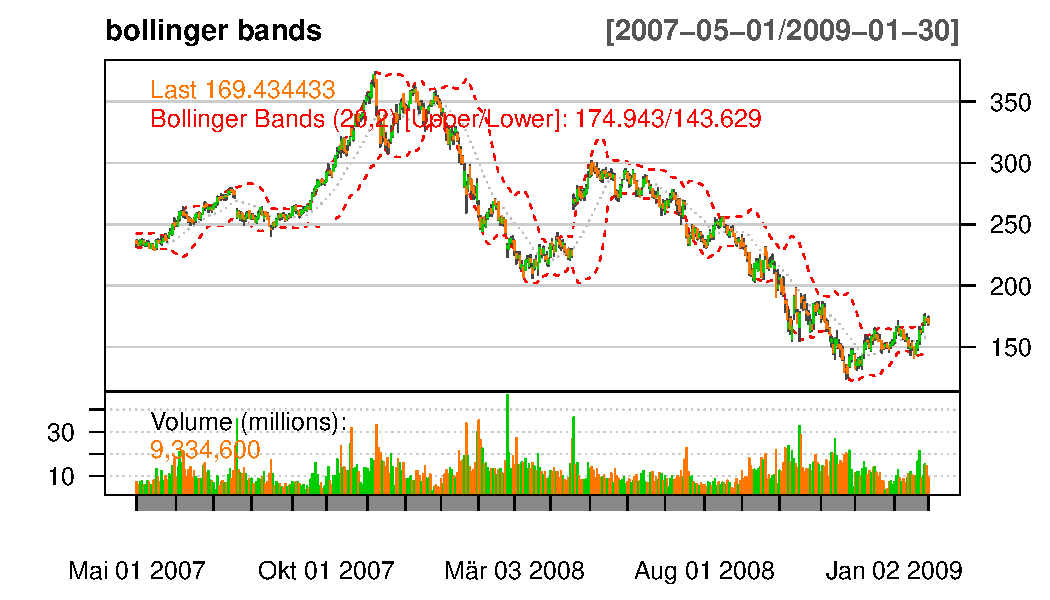
\includegraphics[width=0.7\linewidth]{00_main_files/figure-latex/chap2.6 -1} 

}

\caption{Bollinger Bands}\label{fig:chap2.6 }
\end{figure}
\newpage

\hypertarget{sharpe-ratio}{%
\subsubsection{2.7. Sharpe Ratio}\label{sharpe-ratio}}

Sharpe ratio is a very powerful and widely used ratio to measure
performance. It describes return per risk.

\begin{equation}
  \label{eq:Sharperatio}
  \mathrm{SharpeRatio}=\frac{R_{p}-R_{f}}{\sigma}
\end{equation}

\begin{itemize}
\tightlist
\item
  \({R_p}\) = Return of Portfolio
\item
  \({R_p}\) = Risk free Rate, mostly treasury bonds
\item
  \({\sigma_p}\) = standard deviation of portfolios excess return (risk)
\end{itemize}

\hypertarget{carry}{%
\subsubsection{2.8. Carry}\label{carry}}

Carry trades are trading strategies were usually money is borrowed at a
lower interest rate, than the investment is giving in return. the risk
of this strategy is based in the currency risk.

\newpage

\newpage

\hypertarget{methodology}{%
\subsection{3. Methodology}\label{methodology}}

In this section models are created, trying to outperform the buy and
hold strategy. starting by analyzing the data and using simple models,
more complex models and combined tools are added step by step in
different approaches.

\hypertarget{data-analysis-1}{%
\subsubsection{3.1. Data Analysis}\label{data-analysis-1}}

As mentioned in section \protect\hyperlink{ts-analysis}{1.1} We are now
going to analyze the data further to gain as much information as
possible just by using some simple tools and comparisons.

\hypertarget{correlation}{%
\paragraph{3.1.1. Correlation}\label{correlation}}

~

One could nearly tell just by looking at the indexes how strong they're
correlated. The correlation matrix confirms the assumption, the
correlation is nearly 1 for every index to each other.

\begin{table}[!h]

\caption{\label{tab:chap3.1.1.}Correlations oft the four indexes}
\centering
\begin{tabular}[t]{lrrrr}
\toprule
  & Index 1 & Index 2 & Index 3 & Index 4\\
\midrule
\cellcolor{gray!6}{Index 1} & \cellcolor{gray!6}{1.0000000} & \cellcolor{gray!6}{0.9899111} & \cellcolor{gray!6}{0.9788826} & \cellcolor{gray!6}{0.9672956}\\
Index 2 & 0.9899111 & 1.0000000 & 0.9975499 & 0.9921171\\
\cellcolor{gray!6}{Index 3} & \cellcolor{gray!6}{0.9788826} & \cellcolor{gray!6}{0.9975499} & \cellcolor{gray!6}{1.0000000} & \cellcolor{gray!6}{0.9983460}\\
Index 4 & 0.9672956 & 0.9921171 & 0.9983460 & 1.0000000\\
\bottomrule
\end{tabular}
\end{table}

\hypertarget{transformation-volatility-and-clusters}{%
\paragraph{3.1.2. transformation, volatility and
clusters}\label{transformation-volatility-and-clusters}}

~

Applying the natural logarithm to the series is an approach to cancel
out increasing volatility \ref{fig:chap3.1.2.}. The strong upward is
still visible the original series more than doubled its original price
over the whole timespan(index 4)\ref{fig:chap1.1}.

\textbackslash begin\{figure\}

\{\centering \includegraphics[width=0.7\linewidth]{00_main_files/figure-latex/chap 3.1.2. -1}

\}

\textbackslash caption\{Visualization
log\_indizes\}\label{fig:chap 3.1.2. } \textbackslash end\{figure\}

\newpage

By taking the returns of the transformed series we can visualize
volatility clusters as seen in figure. The first value of the series is
eliminated because of the differences \ref{fig:chap3.1.3.}, Clearly
visible are the high spikes in the times of the financial crisis
2007-2009. Also at the end of the series the impact of covid 19 in march
2020 is remarkable.\\
the unconditional volatility of the indexes are
\textcolor{black}{5328.205}, \textcolor{red}{23203.62},
\textcolor{green}{45321.87}, \textcolor{blue}{69771.43}. Which means the
the index 1 is as much as 13 times volatiler than the fourth index.

\begin{figure}

{\centering \includegraphics[width=0.7\linewidth]{00_main_files/figure-latex/chap 3.1.2-1} 

}

\caption{Log returns}\label{fig:chap 3.1.2}
\end{figure}

Applying the natural logarithm to the series is an approach to cancel
out increasing volatility \ref{fig:chap3.1.2}. The strong upward is
still visible the original series more than doubled its original price
over the whole timespan (index 4) \ref{fig:chap1.1}.

\begin{figure}

{\centering 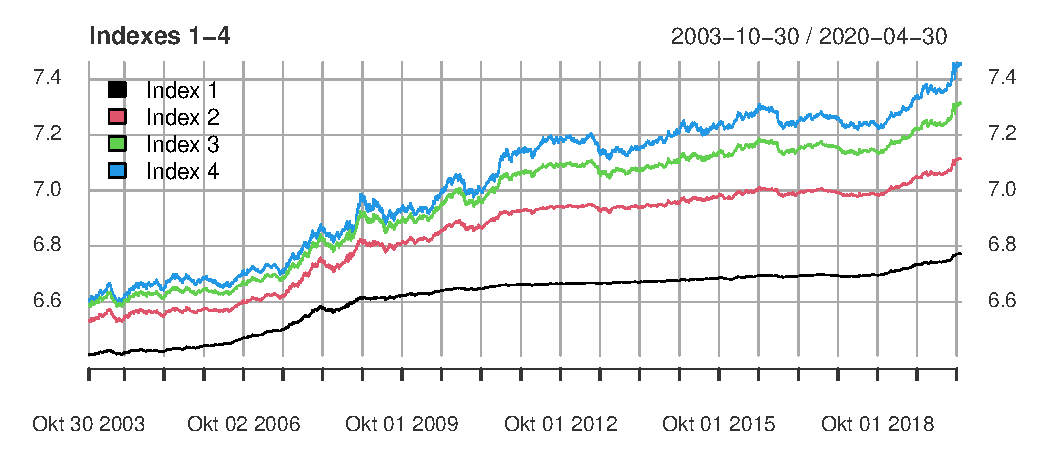
\includegraphics[width=0.7\linewidth]{00_main_files/figure-latex/chap3.1.2-1} 

}

\caption{Visualization log indizes}\label{fig:chap3.1.2}
\end{figure}

\newpage

\hypertarget{autocorrelation-of-log-returns}{%
\paragraph{3.1.2.1 Autocorrelation of log
returns}\label{autocorrelation-of-log-returns}}

~

By computing the acf of the squared log\_returns we see that the
volatility cluster have very long dependency structures.

\begin{figure}

{\centering \includegraphics[width=0.7\linewidth]{00_main_files/figure-latex/chap 3.1.2.1-1} 

}

\caption{ACF log returns}\label{fig:chap 3.1.2.1}
\end{figure}

For further analysis we concentrate on different timespans, because in
most models it makes few sense to consider the whole timeseries from
2003 till today

By taking the returns of the transformed series we can visualize
volatility clusters as seen in figure. The first value of the series is
eliminated because of the differences \ref{fig:chap3.1.3}, Clearly
visible are the high spikes in the times of the financial crisis
2007-2009. Also at the end of the series the impact of covid 19 in march
2020 is remarkable.\\
the unconditional volatility of the indexes are
\textcolor{black}{0.64e-06}, \textcolor{red}{4..1e-06},
\textcolor{green}{8.5e-06}, \textcolor{blue}{15.6e-06}. Which means the
the index 1 is as much as 24 times volatiler than the fourth index.

~

\begin{figure}

{\centering 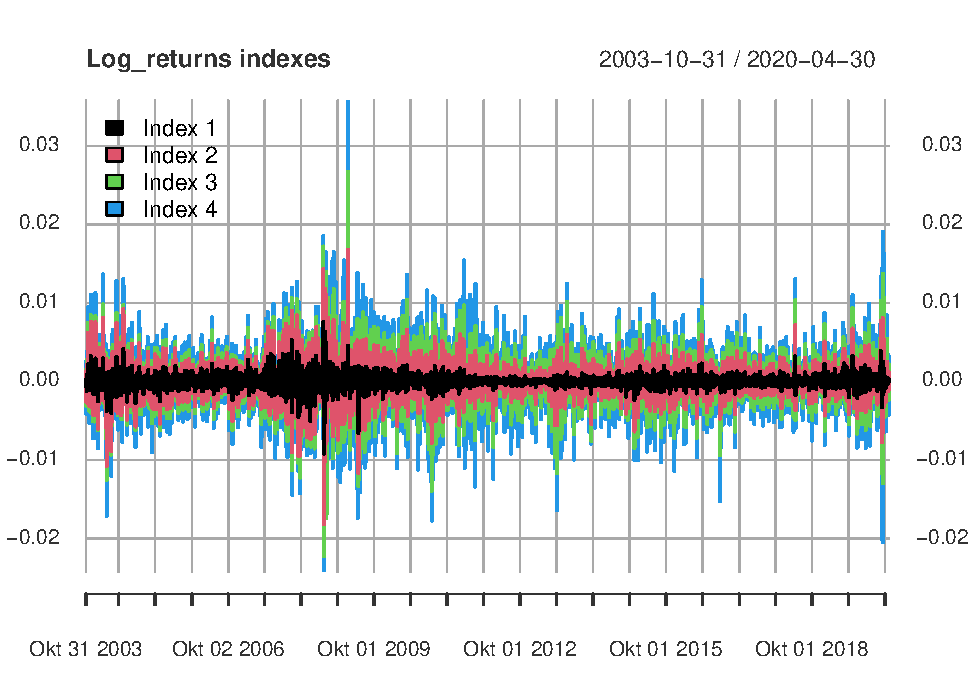
\includegraphics[width=0.7\linewidth]{00_main_files/figure-latex/chap3.1.3-1} 

}

\caption{Log returns}\label{fig:chap3.1.3}
\end{figure}

\newpage

\newpage

\hypertarget{periodicity}{%
\paragraph{3.1.2.2. periodicity}\label{periodicity}}

~

\newpage

~

in Section 2 we have learned different indicators and models for
timeseries-analysis. These models and indicators are now used to trade
the indexes we've introduced in the previous section.

To do so we need to create trading signals based on the models and
indicators. For example we're using the MA Crossings, as mentioned
\protect\hyperlink{Maux5cux2520crossings}{2.3.3.} the points where the
two MAs cross, are now used to create a trading signal. when the longer
MA comes from below to the crossing we are going long the asset and if
it approaches the point from above we're shorting the position.
Technically we apply a 1 to a vector at each crossing, where we intend
to buy and apply a -1 at the points we want to sell.

\hypertarget{buy-and-hold-performance}{%
\subsubsection{3.2.1. Buy and hold
Performance}\label{buy-and-hold-performance}}

~

As mentioned earlier the goal of this work is to outperform the buy and
hold strategy. because the series all have a strong upward trend this
task is very tricky. Buy and hold has very low trading costs because the
underlyings are just bougth once. According to swissquote {[}12{]} costs
for asset trades over 50k are 190 USD per trade \(_1\), so these costs
must also be taken in consideration for the strategy.

\(_1\) notice: This fee is only for private investors, conditions may
differ for institutions.

\hypertarget{portfolios}{%
\paragraph{3.2.1.1 portfolios}\label{portfolios}}

By targeting the best sharpe ratio for the indexes we build a portfolio
for those 4 indexes. One approach would be the equally weighted
portfolio with weights for every index of \(\frac{1}{4}\). As we've seen
in figure \ref{fig:chap3.1.3} the volatility of the indexes strongly
differ, meaning that the index 4 would have the most impact on the
portfolio by weighting it equally. THe cancel out this effect, we're
going to size the position with the inverse volatility, by standardizing
the conditional variance:

\begin{equation}
  \label{eq:standardizing vola}
 standardized\sigma_k = \frac{\sigma_k}{\sum_{k=1}^{4}\sigma_k
\end{equation}

\newpage

\hypertarget{sma-signals-to-trade}{%
\subsubsection{3.2.2. sma signals to trade}\label{sma-signals-to-trade}}

~

As a fisrt approch we apply a moving averag crossing to the timeseries.
The trading horizont is from

\begin{figure}

{\centering \includegraphics[width=0.7\linewidth]{00_main_files/figure-latex/chap3.2.2. ma crossover-1} 

}

\caption{conversion data}\label{fig:chap3.2.2. ma crossover}
\end{figure}

\begin{figure}

{\centering \includegraphics[width=0.7\linewidth]{00_main_files/figure-latex/chap3.2.3. ma crossover-1} 

}

\caption{conversion data}\label{fig:chap3.2.3. ma crossover}
\end{figure}

\newpage

\hypertarget{conclusion}{%
\subsection{4. Conclusion}\label{conclusion}}

In figure \ref{fig:chap4.1} Index 1

\begin{figure}

{\centering \includegraphics[width=0.7\linewidth]{00_main_files/figure-latex/chap4.1-1} 

}

\caption{Index 1.}\label{fig:chap4.1}
\end{figure}

In figure \ref{fig:chap4.2} Index 2

\begin{figure}

{\centering \includegraphics[width=0.7\linewidth]{00_main_files/figure-latex/chap4.2-1} 

}

\caption{Index 2.}\label{fig:chap4.2}
\end{figure}

\newpage

In figure \ref{fig:chap4.3} Index 3

\begin{figure}

{\centering \includegraphics[width=0.7\linewidth]{00_main_files/figure-latex/chap4.3-1} 

}

\caption{Index 3.}\label{fig:chap4.3}
\end{figure}

In figure \ref{fig:chap4.4} Index 4

\begin{figure}

{\centering \includegraphics[width=0.7\linewidth]{00_main_files/figure-latex/chap4.4-1} 

}

\caption{Index 4.}\label{fig:chap4.4}
\end{figure}

\newpage

\hypertarget{references}{%
\subsection{5. References}\label{references}}

\hypertarget{refs}{}
\begin{cslreferences}
\leavevmode\hypertarget{ref-eco1}{}%
{[}1{]} M. Wildi, \emph{Econometrics 1: Time series analysis}.
Winterthur: ZHAW, 2017, p. 221.

\leavevmode\hypertarget{ref-slide_eco3_1}{}%
{[}2{]} M. Wildi, \emph{Econometrics 3: Conditional heteroscedasticity
models, part 1}. ZHAW, 2020, p. 56.

\leavevmode\hypertarget{ref-acf}{}%
{[}3{]} A. H. A. L. Kholkin D. A. Kiselev, \emph{Encyclopedia of
materials: Science and technology (second edition)}. Elsevier, 2001, p.
10388.

\leavevmode\hypertarget{ref-arima}{}%
{[}4{]} M. Masum, ``Time series analysis: Identifying ar and ma using
acf and pacf plots.''
\url{https://towardsdatascience.com/identifying-ar-and-ma-terms-using-acf-and-pacf-plots-in-time-series-forecasting-ccb9fd073db8}
(accessed Nov. 16, 2020).

\leavevmode\hypertarget{ref-garch11}{}%
{[}5{]} B. Williams, \emph{GARCH(1,1) models}.
Ruprecht-Karls-Universität Heidelberg, 2011, p. 42.

\leavevmode\hypertarget{ref-eco2}{}%
{[}6{]} M. Wildi, \emph{An introduction to conditional volatility
models}. Winterthur: ZHAW, 2020, p. 32.

\leavevmode\hypertarget{ref-slide_eco3_3}{}%
{[}7{]} M. Wildi, \emph{Econometrics 3: Conditional heteroscedasticity
models, part 3}. ZHAW, 2020, p. 53.

\leavevmode\hypertarget{ref-SMA}{}%
{[}8{]} A. Hayes, ``Simple moving average.''
\url{https://www.investopedia.com/terms/s/sma.asp} (accessed Sep. 22,
2020).

\leavevmode\hypertarget{ref-EMA}{}%
{[}9{]} A. Hayes, ``Exponential moving average.''
\url{https://www.investopedia.com/terms/e/ema.asp} (accessed Sep. 10,
2020).

\leavevmode\hypertarget{ref-slide_trading_indicators_univariate}{}%
{[}10{]} M. Wildi, \emph{Econometrics 2: Trading indicators}. ZHAW,
2020, p. 78.

\leavevmode\hypertarget{ref-RSI}{}%
{[}11{]} J. Fernando, ``Relative strength index (rsi).''
\url{https://www.investopedia.com/terms/r/rsi.asp} (accessed Nov. 30,
2020).

\leavevmode\hypertarget{ref-swissquote}{}%
{[}12{]} swissquote, ``Trading fees.''
\url{https://library.swissquote.com/shared-images/brochure-trading-pricing-bank-de?_ga=2.183413157.222455671.1606673517-1327743316.1606673517}
(accessed Nov. 29, 2020).
\end{cslreferences}

\newpage

\hypertarget{attachment}{%
\subsection{Attachment}\label{attachment}}

\end{document}
